\documentclass[twocolumn]{article}
\usepackage{amsmath,graphicx,float}
\usepackage[mathscr]{euscript}
\title{Finite Difference Time Domain Analysis of the Electromagnetic Field of a Dipole Antenna}
\author{Tucker DiNapoli}
\date{\today}
\begin{document}
\maketitle
\begin{abstract}
\textbf{This paper provides a basic introduction to the Finite-Difference Time-Domain technique for solving
partial differential equations, specifically its use in computational electrodynamics. The basic idea
of the technique is outlined before a more in depth derivation using the underlying physics. An
example problem of a simple dipole antenna is used as a practical demonstration of the
technique. The software used (openEMS) is discussed and the data generated for the dipole antenna
problem is presented.}
\end{abstract}
\\ \\ \\
%introduction
\def\thesection{\Roman{section}.}
\section{Introduction and History}

There are many problems in electromagnetism which can not be solved using analytic means, likewise
there are many numerical methods available which can be used to calculate approximate solutions with
very high precision. This paper will cover one of these methods, the Finite-Difference Time-Domain
(FDTD) method. The basic ideas behind the method will be covered followed by a more comprehensive
overview including the requisite physics. Following the explanation of the method will be a
practical demonstration of modeling the electromagnetic fields generated by a dipole antenna using
the openEMS software\cite{openEMS}. After an overview of the physics behind the problem the data
generated by FDTD will be given in the form of plots showing the fields and how they evolve over
time. Finally the paper concludes with %something...
%numerical methods overview

FDTD approximates the continuous electromagnetic fields as a series of finite points in time, thus
the name Finite Difference Time Domain. At the core of the method lies the idea of numerical
differentiation where the derivative is calculated as a function of the surrounding points, a simple
formula for numerical differentiation is given by:
\begin{equation} \label{center}
f'(x)=\frac{f(x+h)-f(x-h)}{2h}+\mathscr{O}(h^2)
\end{equation}
where h is the separation between points, a small value of h will give more accurate results. While
there are finite difference equations that give higher accuracy however these require more points
and take longer to compute and so \eqref{center} is the equation used in FDTD. In its simplest form
FDTD uses \eqref{center} to discretize Maxwell equations and then computes the fields by finding the
values of the fields at discrete points using the derived equations. This tactic makes FDTD one of
the easiest algorithms to implement in computational electrodynamics, yet the underlying physics are
still quite complex and it can be expensive to compute.\cite{ebook}
%FDTD, yee blocks, boundry conditions, physics, all of that kinda stuff

The FDTD method was first proposed by Yee in \cite{yee66} as a method for solving scattering
problems based on Maxwell's equations. The method was not widely used until the early 1980s because
of a combination of a lack of computational resources and difficultly in dealing with boundary
conditions. The introduction of absorbing boundary conditions(ABC) by Mur \cite{abcsimple} lead to
increased use of the and further development of the technique. The next major advancement in FDTD
came with Berenger's perfectly matched layer's(PML) boundary conditions \cite{berenger-pml} in the
mid 1990s. In the past 2-3 decades as powerful computational resources have become more affordable
and accessible the use of FDTD has increased dramatically because of its ease of use and
implementation.

\section{Derivation}
FDTD is based on two of Maxwell's equations,
\begin{equation} \label{faraday}
\nabla\times\mathbf{\bar{E}}=-\frac{\partial\mathbf{\bar{B}}}{\partial t}\qquad \text{(Faraday's law)}
\end{equation}
\begin{equation} \label{ampere}
\nabla\times\mathbf{\bar{H}}=\frac{\partial\mathbf{\bar{D}}}{\partial t}+\bar{\mathbf{J}}
\qquad \text{(Amp}\grave{\mathrm{e}}\text{re's Law)}
\end{equation}
In order to transform \eqref{faraday} and \eqref{ampere} into a form that can be evaluated by a
computer they must be rewritten in a form that acts on discrete points. To do this a mesh is created
with a time-step $\delta{t}$ and a spacial step $\delta=\delta{x}=\delta{y}=\delta{z}$ such that any
point $(i,j,k)=(i\delta,j\delta,k\delta)$ and a function $F(i\delta,j\delta,k\delta,n\delta
{t})=F^n(i,j,k)$ \cite{yee66}.\footnote{$\delta$ has been set to the same value for x,y\&z as this
  is often the case and it simplifies much of the math, however in order to maintain generality
  several equations will be presented preserving $\delta{x},\delta{y}\&\delta{z}$ as separate
  values.} The domain for the FDTD calculation now consists of n $\delta\times\delta\times\delta$
cells, the composition of one cell is shown below in figure 1.

\begin{figure}[h]
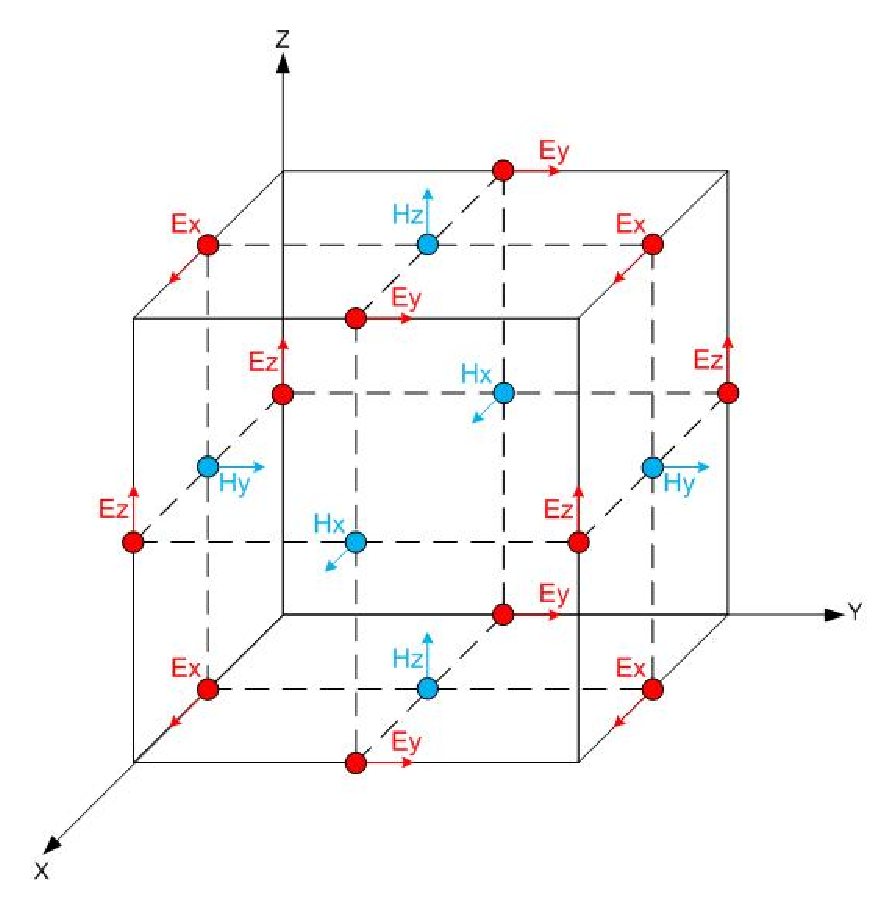
\includegraphics[keepaspectratio,width=\linewidth]{YeeCell01}
\caption{One cell from the mesh used in FDTD showing the relative positions and orientations of the E\&H fields}
\end{figure}\footnote{picture taken from \cite{wiki} and licensed under a creative commons attribution share-alike license}
To calculate E\&H on this mesh \eqref{faraday} and \eqref{ampere} must be expanded into six scalar
equations and the partial derivatives discretized as in \eqref{center}.This leads to the six
equations actually used in FDTD calculations, the equations for the x components are given below,
all six equations along with a more through derivation beyond the scope of this paper can be found
in \cite{parallel}.
\begin{multline} \label{Hx}
H_x^{n+1/2}(i,j+\frac{1}{2},k+\frac{1}{2})=H_x^{n-1/2}(i,j+\frac{1}{2},k+\frac{1}{2})\\
+\frac{\Delta{t}}{\mu_0\cdot\Delta{z}}*[E_y^n(i,j,k+\frac{1}{2})-E_y^n(i,j,k-\frac{1}{2})]\\
-\frac{\Delta{t}}{\mu_0\cdot\Delta{y}}*[E_z^n(i,j+1,k+\frac{1}{2})-E_z^n(i,j,k+\frac{1}{2})]
\end{multline}

\begin{multline} \label{Ex}
E_x^{n}(i+\frac{1}{2},j,k)=E_x^{n-1/2}(i+\frac{1}{2},j,k)\\
+\frac{\Delta{t}}{\epsilon_0\cdot\Delta{y}}*[H_z^n(i+\frac{1}{2},j+\frac{1}{2},k)\\
-H_z^{n-1/2}(i+\frac{1}{2},j-\frac{1}{2},k)]\\
-\frac{\Delta{t}}{\epsilon_0\cdot\Delta{z}}*[H_y^{n-1/2}(i+\frac{1}{2},j,k+\frac{1}{2})\\
-H_y^{n-1/2}(i+\frac{1}{2},j,k-\frac{1}{2})]
\end{multline}
\footnote{Looking at the above equations the fact that there are time and space steps of
  $\frac{1}{2}$ may seem odd. These are a side effect of the Yee lattice and are dealt with in
  practice by setting the E\&H fields a half-step apart and thus removing the factor of
  $\frac{1}{2}$ from the calculations.  In order for the method to work there is a minimum $\delta$
  value that must be chosen so that}

\begin{subequations}\label{step-size}
\begin{align}
c_0\delta{t}\leq\sqrt{\delta{x^{-2}}+\delta{y^{-2}}+\delta{z^{-2}}}\\
c_0\delta{t}\leq\frac{1}{\delta}\label{stability}
\end{align}
\end{subequations}
where $c_0$ is the speed of light. Looking at \eqref{stability}, the one dimensional case, it is
easy to seen that if this condition did not hold (i.e. $c_0\delta{t}<\frac{1}{\delta}$) that the
wave would have to travel faster than light to cover the distance $\delta$ in the time $\delta{t}$,
which would violate causality.

%boundry conditions
The main complication of FDTD is in dealing with boundary conditions, that is how to calculate the
fields in the cells that compose the exterior of the mesh,specifically the electric field being as
the magnetic field is calculated in the center of a cell. There are three main types of boundary
conditions that have been used in FDTD over time, though in practice only the newest of these is
used. They are the perfect conductor, the absorbing boundary condition and the perfectly matched
layers. The idea of a perfect conductor is simple, the boundary cells are calculated by assuming
they are bordered by a perfect conductor. This was the type of boundary condition used in the
initial formulations of the FDTD methods and rarely used in practice\cite{parallel}.Absorbing
boundary condition-(ABC) were first developed by Mur in \cite{abcsimple}, where a much more through
and complete derivation and analysis can be found. ABC assumes that the boundary is composed of an
absorbing material and calculates the E field using this assumption.In a one dimensional ABC can be
given by the equation:
\begin{equation}\label{ABC}
E_{x=0}^{t=1}=E_{x=-1}^{t=0}+\frac{c_0\delta{t}-\delta{x}}{c_0\delta{t}+\delta{x}}[E_{x=0}^{t=0}+E_{x=-1}^{t=1}]\\
\text{where the boundry is x=0 starting at x=-1 and t=0}
\end{equation}
looking at this equation E at the boundary is determined by averaging what the value of E will be at
the current position one step forward in time and the value of E at the boundary at the current
time. These two values are obtained by assuming E satisifys the wave equation at the boundary and
calculating the approximate values from this. Absorbing boundary conditions can be made more
accurate by calculating these values as a second order approximation, ABC methods were the
predominant boundary conditions used in FDTD from their development in the early 1980s until the
advent of the method of perfectly matched layer(PML). The PML technique was developed by Berenger in
\cite{berenger-pml} and works by assuming the boundary is composed of a theoretical PML medium whose
properties are defined through a series of equations defining how the E\&H fields interact with
it. The PML technique is very complex and was developed in such a way as to maximize accuracy of
FDTD techniques. It is the most widely used boundary condition in FDTD analysis,for a more through
and mathematical analysis of the technique see\cite{berenger-pml}or\cite{parallel}.
\section{Dipole Antenna Problem}

%Dipole Antenna, overview of the problem
The problem to be modeled is calculating the fields generated from an idealized half-wave dipole
antenna. A dipole antenna is one of the simplest forms of antennas and consists of 2 sections of
wire (or other conducting material) in line with each other with a small gap in between them where
an oscillating voltage is applied. While the wires can be of any length most often the two wires
will each have a length $\Lambda/4$ giving a total length $\Lambda/2$ thus a half-wave antenna. The
only type of dipole antenna for which the fields can be exactly solved is the physically impossible
case of the elementary doublet, consisting of a wire of length $\delta{l}$ where
$\delta{l}<<\Lambda$ through which an alternating current is run. This situations is impossible
because realistically there must be a current source. The next most simple dipole antenna is a short
dipole consisting of two separate wires and containing a current source, but still with length
$\delta{l}$. While the short dipole makes calculations easy it makes for an inefficient antenna,
which is why the half-wave antenna is the type of dipole antenna most often used, and why methods
for calculating the electromagnetic fields from it are important. Despite this the problem looked at
in this paper is an idealized antenna, essentially an elongated elementary doublet. The goal of this
paper is not in solving a complicated problem but showing how FDTD works and why it is useful.

\section{Computation}
The author had originally intended to write an FDTD program himself however after looking at several
open source FDTD programs and libraries decided the task was beyond the scope of this report. FDTD
simulation is a very computationally intensive process, requiring large amounts of memory to store
the information about the fields and a significant amount of processing power to run through the
large number of calculations that must be done. There are several software packages available for
FDTD simulation, both commercial and open-source software. Two pieces of software were considered
for the FDTD simulation, Meep an open source FDTD solver developed at MIT and written in c++ and
openEMS which is another open source FDTD solver written in c++ which also has a matlab/octave
interface. OpenEMS was used for this paper because it proved easier to use than meep and allowed for
the easy creation of graphics.

OpenEMS takes an xml file containing information about the geometry and material properties of the
system being modeled. This input allows for the creation of complicated geometries with linear and
nonlinear materials, showing the versatility of the FDTD technique. It uses this input to start an
FDTD simulation which it records in a series of hdf5 data-files. It has the ability to generate
information about the far fields from the FDTD simulation, something not available with FDTD
modeling as it relies on iterative methods. The file used in modeling is a modified version of an
infinite dipole script included with the package. Several aspects have been modified to created a
script simulating a half-wave dipole antenna. As the goal is to provide a simple example and
understand the method the simulation is run as if the dipole was in a vacuum, and as previously
stated as if there were no current source.

%Data, plots and such generated by FDTD
There is a large ammount of data generated from an FDTD simulation, there is information on each of
the components of the E and H fields in each cell of the entire lattice making for a lot of data. In
openEMS this data is stored in hdf5 files , the hdf5 format is a format designed to hold large
ammount of scientific or numerical data in a compressed and organized fashion\cite{hdf5}. For the
FDTD analysis run two hdf5 files for each component of each field were generated, each about 9
megabytes, showing the sheer ammount of data that FDTD uses and generates, being as the focus of this
paper is not on data analysis this data is not used. The data that is presented are octave plots of
the far fields generated from openEMS,which are extensions of the FDTD output, and a sample of the
output from openEMS included at the end of the document.
\section{Data}
%octave plots
\begin{figure}[p,h!]
\vspace{-20pt}
\includegraphics[keepaspectratio,width=\linewidth]{far0}
\caption{A view of the electric far field at $\phi=0^{\circ}$ in spherical coordinates}
\end{figure}

\begin{figure}[p,h]
\includegraphics[keepaspectratio,height=0.4\textheight,width=\linewidth]{far90}
\caption{A view of the electric far field at $\phi=90^{\circ}$ in spherical coordinates}
\end{figure}

\begin{figure}[p,h]
\includegraphics[keepaspectratio,height=0.4\textheight,width=\linewidth]{far180}
\caption{A view of the electric far field at $\phi=180^{\circ}$ in spherical coordinates}
\end{figure}

\section{Conclusion}
%Conclusion
This paper has only been a brief overview of the FDTD method, it is an incredibly versatile methods
with many different implementations. The popularity of the FDTD method means improvements and
modifications to the technique are being developed rapidly. For instance \cite{ADI} describes an
application of the technique using implicit differentiation, resulting in more computationally
intensive calculations but with the benefit of being unconditionally stable(i.e. there is no maximum
time step). When compared to two other popular methods in computational electrodynamics, the method
of moments technique(MoM) and the finite element method(FEM) FDTD has obvious strengths and
weaknesses. the MoM technique is different from either FEM or FDTD in that it relies on an integral
methods as opposed to derivative methods utilized by FEM and FDTD. MoM only requires calculating
boundary values, which makes it effective in problems over a small volume, but in general can only be applied to
problems dealing with linear homogeneous material\cite{other}.The FEM is a differential technique like
FDTD, it deals with dividing the problem up into different sized elements depending on the
variation of the fields using larger elements where the fields are relatively stable and smaller
elements where the fields change rapidly. FEM is generally a much more robust method than FDTD, it
can deal with more complicated geometries and is often seen as more mathematically elegant method
than FDTD\cite{other}. This being said FEM is much more difficult to implement than FDTD, it
requires significantly more computational power than FDTD in electromagnetic problems and is
difficult if not impossible to implement on an individual level. FDTD relative to other techniques
provides a method that is simple enough to implement by one person on a laptop computer and is
accurate enough for the majority of applications.
\bibliographystyle{ieeetr}
\bibliography{E-M-Project}
%openEMS output
\begin{figure*}[p,h!]
\centering
\small
\begin{verbatim}
 ----------------------------------------------------------------------
 | openEMS 64bit -- version v0.0.30
 | (C) 2010-2012 Thorsten Liebig <thorsten.liebig@gmx.de>  GPL license
 ----------------------------------------------------------------------
Create FDTD operator (compressed SSE + multi-threading)
FDTD simulation size: 97x97x97 --> 912673 FDTD cells
FDTD timestep is: 1.44338e-12 s; Nyquist rate: 346 timesteps @1.00119e+09 Hz
Excitation signal length is: 3969 timesteps (5.72876e-09s)
Max. number of timesteps: 50000 ( --> 12.5976 * Excitation signal length)
Create FDTD engine (compressed SSE + multi-threading)
Running FDTD engine... this may take a while... grab a cup of coffee?!?
[@    4s] Timestep:    102 || Speed:   20.9 MC/s (4.360e-02 s/TS) || Energy: ~2.05e-24 (- 0.00dB)
[@    9s] Timestep:    204 || Speed:   19.9 MC/s (4.595e-02 s/TS) || Energy: ~1.22e-24 (- 2.26dB)
[@   18s] Timestep:    408 || Speed:   20.8 MC/s (4.382e-02 s/TS) || Energy: ~2.20e-22 (- 0.00dB)
[@   28s] Timestep:    612 || Speed:   16.3 MC/s (5.601e-02 s/TS) || Energy: ~8.40e-21 (- 0.00dB)
[@   32s] Timestep:    680 || Speed:   14.3 MC/s (6.382e-02 s/TS) || Energy: ~1.70e-20 (- 0.00dB)
[@   42s] Timestep:    884 || Speed:   21.2 MC/s (4.308e-02 s/TS) || Energy: ~1.48e-20 (- 2.93dB)
[@   47s] Timestep:    986 || Speed:   18.9 MC/s (4.826e-02 s/TS) || Energy: ~1.47e-20 (- 2.96dB)
[@   56s] Timestep:   1190 || Speed:   19.6 MC/s (4.657e-02 s/TS) || Energy: ~2.07e-18 (- 0.00dB)
[@ 1m01s] Timestep:   1258 || Speed:   14.9 MC/s (6.116e-02 s/TS) || Energy: ~4.08e-18 (- 0.00dB)
[@ 1m10s] Timestep:   1462 || Speed:   19.6 MC/s (4.668e-02 s/TS) || Energy: ~7.05e-18 (- 0.08dB)
[@ 1m14s] Timestep:   1564 || Speed:   22.6 MC/s (4.030e-02 s/TS) || Energy: ~2.42e-18 (- 4.74dB)
[@ 1m19s] Timestep:   1700 || Speed:   22.8 MC/s (4.001e-02 s/TS) || Energy: ~2.32e-18 (- 4.90dB)
[@ 1m28s] Timestep:   1904 || Speed:   19.9 MC/s (4.584e-02 s/TS) || Energy: ~3.98e-17 (- 0.00dB)
[@ 1m32s] Timestep:   2006 || Speed:   21.9 MC/s (4.176e-02 s/TS) || Energy: ~4.70e-17 (- 0.04dB)
[@ 1m41s] Timestep:   2210 || Speed:   20.8 MC/s (4.390e-02 s/TS) || Energy: ~1.06e-17 (- 6.50dB)
[@ 1m45s] Timestep:   2312 || Speed:   22.0 MC/s (4.147e-02 s/TS) || Energy: ~2.74e-19 (-22.39dB)
[@ 1m50s] Timestep:   2414 || Speed:   19.2 MC/s (4.764e-02 s/TS) || Energy: ~2.65e-18 (-12.53dB)
[@ 1m54s] Timestep:   2482 || Speed:   14.3 MC/s (6.403e-02 s/TS) || Energy: ~6.04e-18 (- 8.95dB)
[@ 2m03s] Timestep:   2686 || Speed:   20.9 MC/s (4.369e-02 s/TS) || Energy: ~5.08e-18 (- 9.70dB)
[@ 2m08s] Timestep:   2788 || Speed:   21.3 MC/s (4.284e-02 s/TS) || Energy: ~1.96e-18 (-13.83dB)
[@ 2m12s] Timestep:   2890 || Speed:   21.9 MC/s (4.169e-02 s/TS) || Energy: ~3.83e-19 (-20.93dB)
[@ 2m17s] Timestep:   2992 || Speed:   18.7 MC/s (4.878e-02 s/TS) || Energy: ~1.20e-20 (-35.98dB)
[@ 2m21s] Timestep:   3094 || Speed:   21.7 MC/s (4.204e-02 s/TS) || Energy: ~1.68e-20 (-34.51dB)
[@ 2m25s] Timestep:   3196 || Speed:   21.3 MC/s (4.284e-02 s/TS) || Energy: ~2.94e-20 (-32.08dB)
[@ 2m30s] Timestep:   3298 || Speed:   21.8 MC/s (4.193e-02 s/TS) || Energy: ~1.67e-20 (-34.52dB)
[@ 2m34s] Timestep:   3400 || Speed:   22.9 MC/s (3.981e-02 s/TS) || Energy: ~5.36e-21 (-39.47dB)
[@ 2m39s] Timestep:   3502 || Speed:   17.9 MC/s (5.090e-02 s/TS) || Energy: ~1.11e-21 (-46.30dB)
[@ 2m44s] Timestep:   3604 || Speed:   19.0 MC/s (4.792e-02 s/TS) || Energy: ~2.11e-22 (-53.52dB)
[@ 2m49s] Timestep:   3706 || Speed:   19.8 MC/s (4.607e-02 s/TS) || Energy: ~9.35e-23 (-57.05dB)
[@ 2m53s] Timestep:   3808 || Speed:   20.5 MC/s (4.447e-02 s/TS) || Energy: ~6.80e-23 (-58.43dB)
[@ 2m58s] Timestep:   3910 || Speed:   21.1 MC/s (4.331e-02 s/TS) || Energy: ~4.99e-23 (-59.78dB)
[@ 3m03s] Timestep:   4012 || Speed:   18.1 MC/s (5.056e-02 s/TS) || Energy: ~3.79e-23 (-60.98dB)
Time for 4012 iterations with 912673.00 cells : 183.19 sec
Speed: 19.99 MCells/s
\end{verbatim}
\caption{Verbatim output from openEMS, with some lines/spaces removed to trim to a reasonable size.}
\end{figure*}
\normalsize
\end{document}

%  LocalWords:  openEMS discretize MoM
